% Fichier pour la visualisation du potentiel hiérarchique
\documentclass[tikz,border=10pt]{standalone}
\usepackage{tikz}
\usepackage{pgfplots}
\pgfplotsset{compat=1.18}
\usetikzlibrary{decorations.pathreplacing,decorations.markings,arrows.meta,calc,3d,backgrounds}
\usepackage{xcolor}

% Définition des couleurs
\definecolor{primaryblue}{RGB}{0,114,178}
\definecolor{secondaryred}{RGB}{213,94,0}
\definecolor{tertiarygreen}{RGB}{0,158,115}
\definecolor{quaternarypurple}{RGB}{86,60,143}

\begin{document}

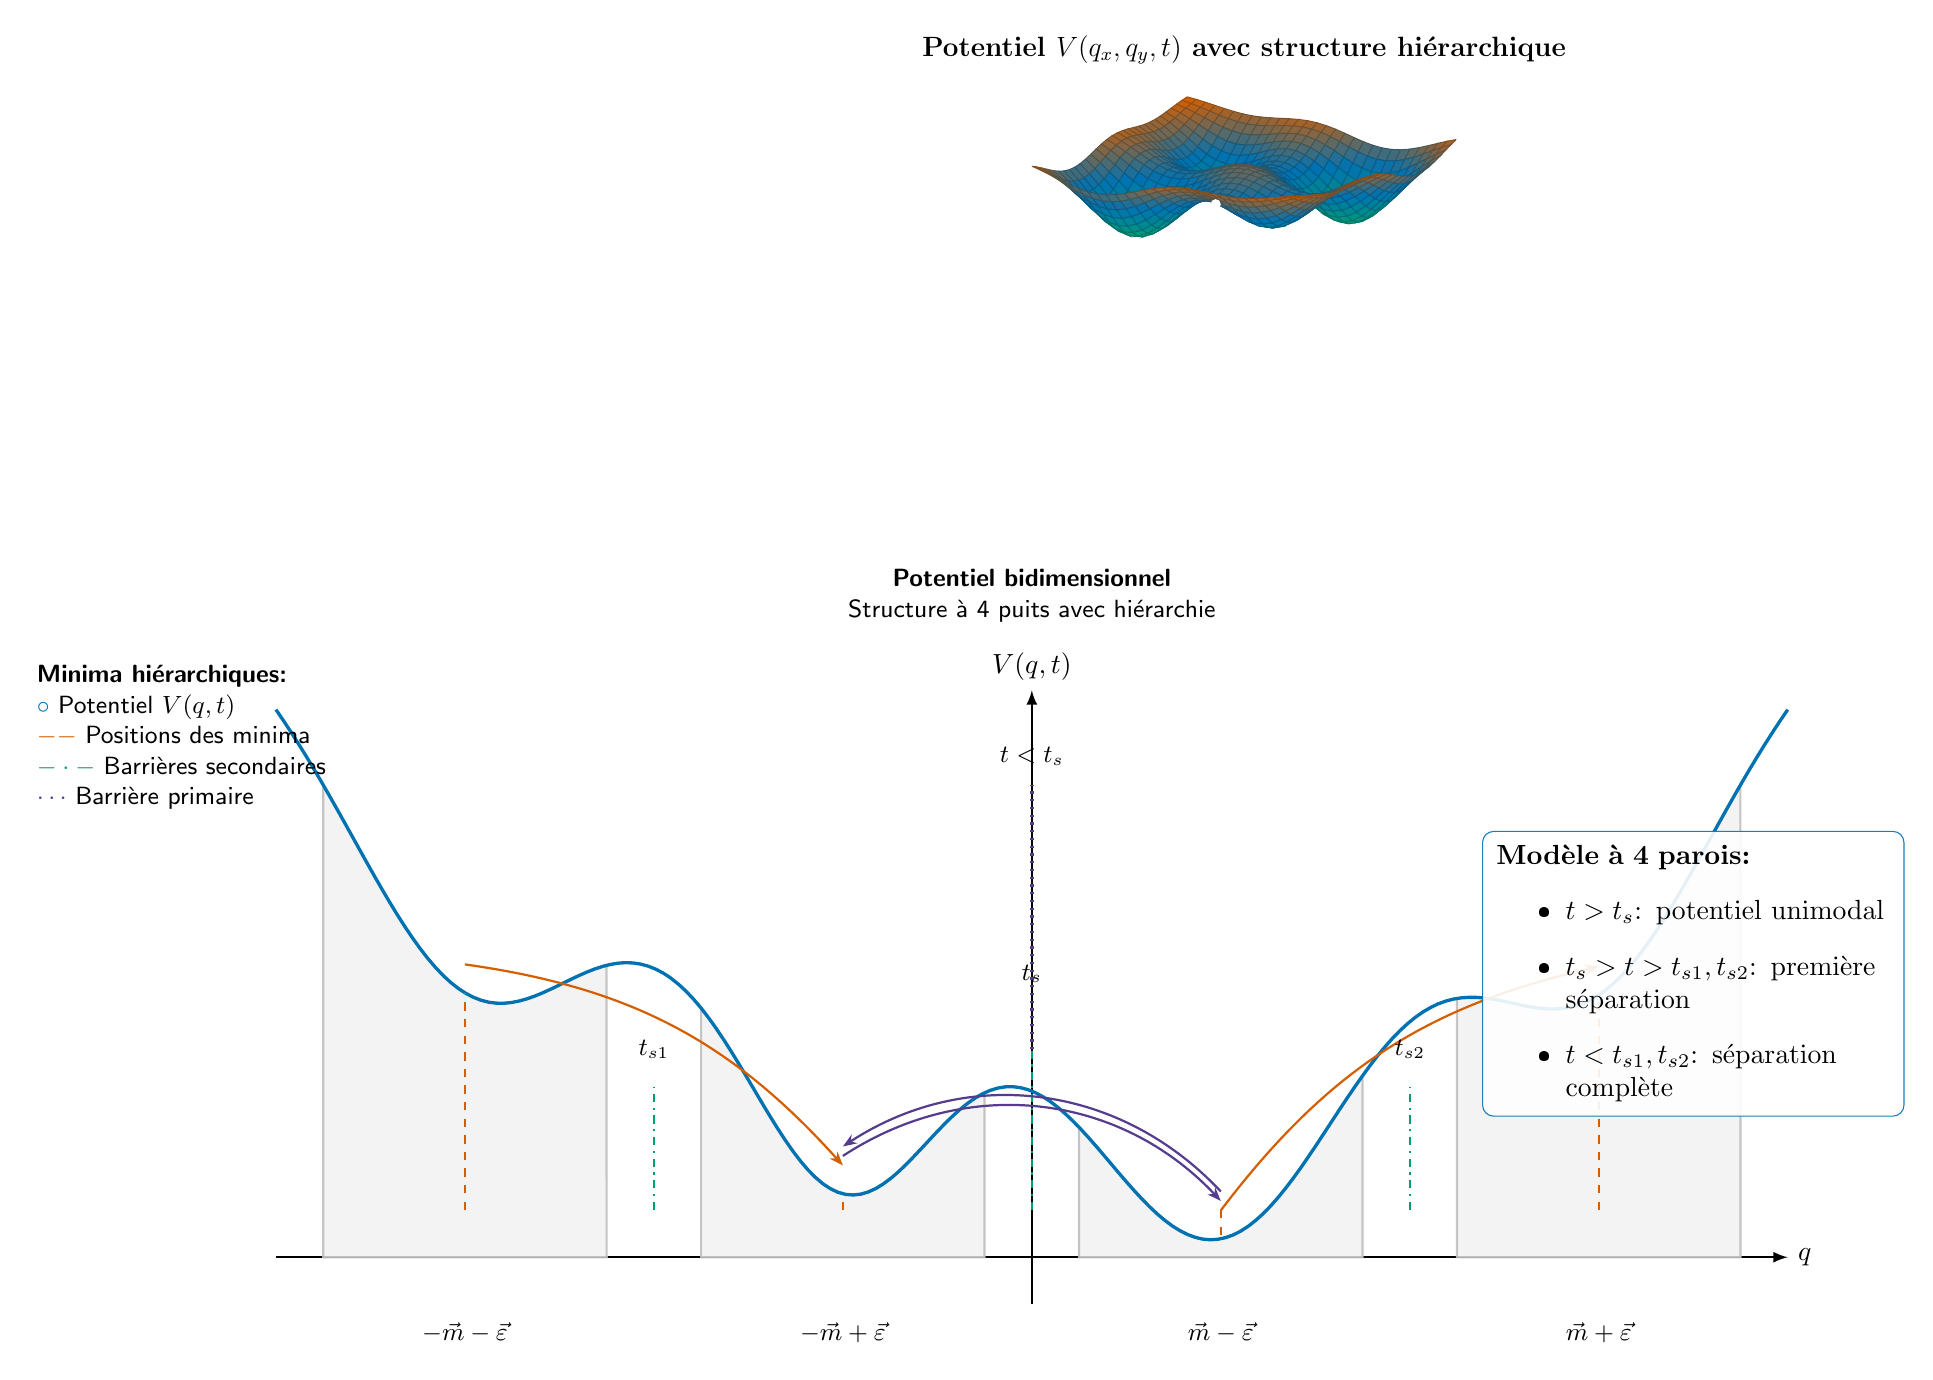
\begin{tikzpicture}[scale=1.2]
% Définition des styles
\tikzset{
    annotation/.style={font=\small\sffamily, text=black, align=center},
    highlight/.style={ultra thick, primaryblue},
    wall/.style={thick, fill=gray!10, draw=gray!50, opacity=0.9},
    arrow/.style={-{Stealth[length=5pt]}, thick},
    level1/.style={thick, secondaryred},
    level2/.style={thick, tertiarygreen},
    level3/.style={thick, quaternarypurple}
}

% Paramètres du graphique
\pgfmathsetmacro{\xmin}{-8}
\pgfmathsetmacro{\xmax}{8}
\pgfmathsetmacro{\ymin}{-0.5}
\pgfmathsetmacro{\ymax}{6}

% Fonction du potentiel (potentiel à 4 parois avec hiérarchie)
\pgfmathdeclarefunction{potentiel}{1}{%
    \pgfmathsetmacro{\resultone}{3 + 0.05*(#1)*(#1) - 2*exp(-0.4*(#1+6)*(#1+6)) - 2.5*exp(-0.5*(#1+2)*(#1+2)) - 3*exp(-0.3*(#1-2)*(#1-2)) - 2*exp(-0.4*(#1-6)*(#1-6))}%
    \pgfmathsetmacro{\resulttwo}{max(\resultone, 0)}%
    \pgfmathparse{\resulttwo}%
}

% Tracé des axes
\draw[thick, -latex] (\xmin,0) -- (\xmax,0) node[right] {$q$};
\draw[thick, -latex] (0,\ymin) -- (0,\ymax) node[above] {$V(q,t)$};

% Tracé des parois du potentiel (zones ombrées)
\begin{scope}
    \draw[wall] plot[domain=-7.5:-4.5, samples=100] (\x, {potentiel(\x)}) -- (-4.5,0) -- (-7.5,0) -- cycle;
    \draw[wall] plot[domain=-3.5:-0.5, samples=100] (\x, {potentiel(\x)}) -- (-0.5,0) -- (-3.5,0) -- cycle;
    \draw[wall] plot[domain=0.5:3.5, samples=100] (\x, {potentiel(\x)}) -- (3.5,0) -- (0.5,0) -- cycle;
    \draw[wall] plot[domain=4.5:7.5, samples=100] (\x, {potentiel(\x)}) -- (7.5,0) -- (4.5,0) -- cycle;
\end{scope}

% Courbe du potentiel
\draw[very thick, primaryblue] plot[domain=\xmin:\xmax, samples=200] (\x, {potentiel(\x)});

% Ajout des niveaux hiérarchiques
\draw[level1, dashed] (-6,0.5) -- (-6,{potentiel(-6)});
\draw[level1, dashed] (-2,0.5) -- (-2,{potentiel(-2)});
\draw[level1, dashed] (2,0.5) -- (2,{potentiel(2)});
\draw[level1, dashed] (6,0.5) -- (6,{potentiel(6)});

% Niveaux de séparation (barrières)
\draw[level2, dashdotted] (-4,0.5) -- (-4,{1.8});
\draw[level2, dashdotted] (0,0.5) -- (0,{2.2});
\draw[level2, dashdotted] (4,0.5) -- (4,{1.8});

% Ligne de séparation principale
\draw[level3, dotted, line width=1.5pt] (0,2.2) -- (0,5);

% Annotations
\node[annotation] at (-6,-0.8) {$-\vec{m} - \vec{\varepsilon}$};
\node[annotation] at (-2,-0.8) {$-\vec{m} + \vec{\varepsilon}$};
\node[annotation] at (2,-0.8) {$\vec{m} - \vec{\varepsilon}$};
\node[annotation] at (6,-0.8) {$\vec{m} + \vec{\varepsilon}$};

\node[annotation] at (0,5.3) {$t < t_s$};

% Légende des parois/minima
\node[annotation, align=left] at (-9, 5.5) {
    \textbf{Minima hiérarchiques:} \\
    \textcolor{primaryblue}{$\circ$} Potentiel $V(q,t)$ \\
    \textcolor{secondaryred}{$--$} Positions des minima \\
    \textcolor{tertiarygreen}{$-\cdot-$} Barrières secondaires \\
    \textcolor{quaternarypurple}{$\cdots$} Barrière primaire
};

% Ajout de flèches de transition
\draw[arrow, secondaryred, bend left=20] (-6,{potentiel(-6)+0.3}) to (-2,{potentiel(-2)+0.3});
\draw[arrow, secondaryred, bend left=20] (2,{potentiel(2)+0.3}) to (6,{potentiel(6)+0.3});

% Flèches de transition principale (traversée de la barrière centrale)
\draw[arrow, quaternarypurple, bend left=40] (-2,{potentiel(-2)+0.4}) to (2,{potentiel(2)+0.4});
\draw[arrow, quaternarypurple, bend right=40] (2,{potentiel(2)+0.5}) to (-2,{potentiel(-2)+0.5});

% Temps critiques
\node[annotation] at (-4, 2.2) {$t_{s1}$};
\node[annotation] at (0, 3) {$t_s$};
\node[annotation] at (4, 2.2) {$t_{s2}$};

% Image 3D du potentiel au-dessus
\begin{scope}[shift={(0,10)}, scale=0.7]
    \begin{axis}[
        hide axis,
        view={30}{30},
        width=8cm,
        height=5cm,
        colormap={custom}{color(0)=(tertiarygreen); color(0.5)=(primaryblue); color(1)=(secondaryred)},
        z buffer=sort,
        title={\large\textbf{Potentiel $V(q_x, q_y, t)$ avec structure hiérarchique}},
    ]
        % Surface paramétrée pour le potentiel 2D
        \addplot3[
            surf,
            domain=-3:3,
            domain y=-3:3,
            samples=30,
            z buffer=sort,
        ] {4 - 3*exp(-((x-1.5)^2 + (y-1.5)^2)/2) - 3*exp(-((x+1.5)^2 + (y+1.5)^2)/2) - 2*exp(-((x-1.5)^2 + (y+1.5)^2)/1.5) - 2*exp(-((x+1.5)^2 + (y-1.5)^2)/1.5)};
        
        % Points des minima
        \addplot3[only marks, mark=*, mark size=2pt, color=white] coordinates {
            (1.5,1.5,0.2) (-1.5,-1.5,0.2) (1.5,-1.5,1) (-1.5,1.5,1)
        };
    \end{axis}
\end{scope}

% Annotations pour la visualisation 3D
\node[annotation, align=center] at (0,7) {
    \textbf{Potentiel bidimensionnel}\\
    Structure à 4 puits avec hiérarchie
};

% Encadré explicatif
\node[draw=primaryblue, rounded corners, text width=5cm, inner sep=5pt, fill=white, opacity=0.9, text opacity=1] at (7, 3) {
    \textbf{Modèle à 4 parois:}
    \begin{itemize}
        \item $t > t_s$: potentiel unimodal
        \item $t_s > t > t_{s1}, t_{s2}$: première séparation
        \item $t < t_{s1}, t_{s2}$: séparation complète
    \end{itemize}
};

\end{tikzpicture}
\end{document}
